\subsection{二阶行列式}
\subsubsection{二元线性方程组}
\paragraph{}
用消元法解二元线性方程组
\begin{align}
\label{消元法解二元线性方程组}
\begin{split}
  \left\{ \begin{array}{l}
    a_{11}x_1 + a_{12}x_2 = b_1, \\
    a_{21}x_1 + a_{22}x_2 = b_2.
  \end{array} \right.
\end{split}
\end{align}

\paragraph{}
为消去未知数$x_2$,以$a_{22}$与$a_{12}$分别乘上列两方程的两端,然后两个方程相减,得
\begin{equation*}
  (a_{11}a_{22} - a_{12}a_{21})x_1 = b_1a_{22} - a_{12}b_2;
\end{equation*}
类似地,消去$x_1$,得
\begin{equation*}
  (a_{11}a_{22} - a_{12}a_{21})x_2 = a_{11}b_2 - b_1a_{21}.
\end{equation*}

\paragraph{}
当$a_{11}a_{22} - a_{12}a_{21} \neq 0$时,求得方程组\eqref{消元法解二元线性方程组}的解为
\begin{equation}
  \label{二元线性方程组的解}
  x_1 = \frac{ b_1a_{22} - a_{12}b_2 }{ a_{11}a_{22} - a_{12}a_{21} }, \; x_2 = \frac{ a_{11}b_2 - b_1a_{21} }{ a_{11}a_{22} - a_{12}a_{21} }.
\end{equation}

\subsubsection{二阶行列式}
\paragraph{}
其中分母$a_{11}a_{22} - a_{12}a_{21}$ 是由方程组\eqref{消元法解二元线性方程组}的四个系数确定的,把这四个数按它们在方程组\eqref{消元法解二元线性方程组}中的位置,排成二行二列的数表
\begin{equation}
\label{二阶数表}
\begin{array}{cc}
a_{11} & a_{12} \\ a_{21} & a_{22},
\end{array}
\end{equation}
表达式$a_{11}a_{22} - a_{12}a_{21}$称为数表\eqref{二阶数表}所确定的\textbf{二阶行列式},并记作
\begin{equation}
  \left|
  \begin{array}{cc}
  a_{11} & a_{12} \\ a_{21} & a_{22}
  \end{array} \right|.
\end{equation}

\subsubsection{对角线法则}
\paragraph{}
二阶行列式的定义,可以用\textbf{对角线法则}来记忆。$a_{11}$到$a_{22}$的实线称为\textbf{主对角线},$a_{12}$到$a_{21}$的虚线称为\textbf{副对角线}。于是二阶行列式便是:主对角线上的两元素之积减去副对角线上的两元素之积所得的差。
\begin{figure}[H]
\centering
  % 二阶行列式的对角线法则
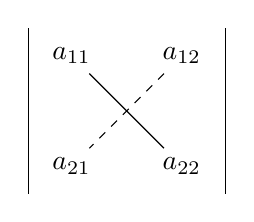
\begin{tikzpicture}
  \draw (-1.25,1.05) -- (-1.25,-1.05);

  \node at (-.7,.7) (a11) {$a_{11}$};
  \node at (.7,-.7) (a22) {$a_{22}$};
  \draw (a11) -- (a22);

  \node at (.7,.7) (a12) {$a_{12}$};
  \node at (-.7,-.7) (a21) {$a_{21}$};
  \draw[dashed] (a12) -- (a21);

  \draw (1.25,1.05) -- (1.25,-1.05);
\end{tikzpicture}

  \caption{对角线法则}
  \label{图:二阶对角线法则}
\end{figure}

\subsubsection{二元线性方程组的解}
\paragraph{}
利用二阶行列式的概念和对角线法则,\eqref{二元线性方程组的解}式中$x_1,x_2$的分子也可写成二阶行列式,即
\begin{equation*}
  b_1a_{22} - a_{12}b_2 = \left|\begin{array}{cc} b_1 & a_{12} \\ b_2 & a_{22}\end{array}\right|, \;
  a_{11}b_2 - b_1a_{21} = \left|\begin{array}{cc} a_{11} & b_1 \\ a_{21} & b_2\end{array}\right|,
\end{equation*}

\paragraph{}
若记
\begin{equation*}
  D = \left|\begin{array}{cc} a_{11} & a_{12} \\ a_{21} & a_{22} \end{array}\right|, \;
  D_1 = \left|\begin{array}{cc} b_1 & a_{12} \\ b_2 & a_{22} \end{array}\right|, \;
  D_2 = \left|\begin{array}{cc} a_{11} & b_1 \\ a_{21} & b_2 \end{array}\right|, \;
\end{equation*}
那么\eqref{二元线性方程组的解}式可写成
\begin{equation*}
  x_1 = \frac{D_1}{D} = \frac{\left|\begin{array}{cc} b_1 & a_{12} \\ b_2 & a_{22} \end{array}\right|}{\left|\begin{array}{cc} a_{11} & a_{12} \\ a_{21} & a_{22} \end{array}\right|}, \;
  x_2 = \frac{D_2}{D} = \frac{\left|\begin{array}{cc} a_{11} & b_1 \\ a_{21} & b_2 \end{array}\right|}{\left|\begin{array}{cc} a_{11} & a_{12} \\ a_{21} & a_{22} \end{array}\right|}.
\end{equation*}

\paragraph{}
注意,这里的分母$D$是由方程组\eqref{消元法解二元线性方程组}的系数所确定的二阶行列式(称系数行列式),$x_1$的分子$D_1$是常数项$b_1,b_2$替换$D$中$x_1$的系数$a_{11}, a_{21}$(第$1$列)所得的二阶行列式;$x_2$的分子$D_2$是用常数项$b_1, b_2$替换$D$中$x_2$的系数$a_{12}, a_{22}$(第$2$列)所得的二阶行列式。

\subsection{三阶行列式}
\subsubsection{定义}
\paragraph{}
\textbf{定义~~}设有$9$个数排成$3$行$3$列的数表
\begin{equation}
  \label{三阶数表}
  \begin{array}{ccc}
    a_{11} & a_{12} & a_{13} \\
    a_{21} & a_{22} & a_{23} \\
    a_{31} & a_{32} & a_{33},
  \end{array}
\end{equation}
记
\begin{align}
\centering
  \begin{split}
    \label{三阶行列式}
    &\;\left|\begin{array}{ccc}
      a_{11} & a_{12} & a_{13} \\
      a_{21} & a_{22} & a_{23} \\
      a_{31} & a_{32} & a_{33}
    \end{array}\right| \\
    =&\; a_{11}a_{22}a_{33} + a_{12}a_{23}a_{31} + a_{13}a_{21}a_{32} - \\
    &\; a_{11}a_{23}a_{32} - a_{12}a_{21}a_{33} - a_{13}a_{22}a_{31},
  \end{split}
\end{align}
\eqref{三阶行列式}称为数表\eqref{三阶数表}所确定的三阶行列式。

\subsubsection{对角线法则}
\begin{figure}[H]
\centering
  % 三阶行列式的对角线法则
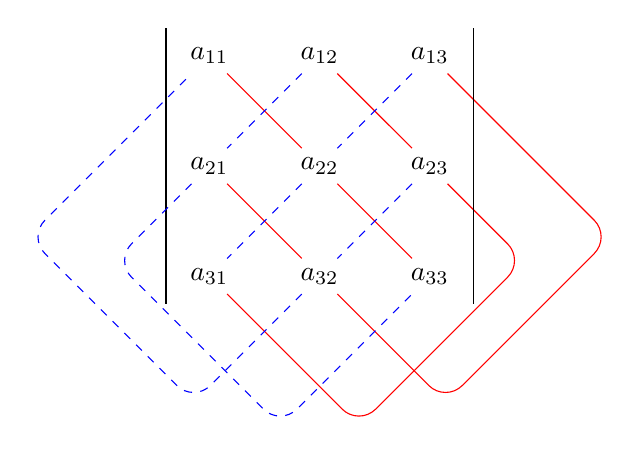
\begin{tikzpicture}

  \draw (-1.95,1.75) -- (-1.95,-1.75);

  \node at (-1.4,1.4) (a11) {$a_{11}$};
  \node at (0,1.4) (a12) {$a_{12}$};
  \node at (1.4,1.4) (a13) {$a_{13}$};

  \node at (-1.4,0) (a21) {$a_{21}$};
  \node at (0,0) (a22) {$a_{22}$};
  \node at (1.4,0) (a23) {$a_{23}$};

  \node at (-1.4,-1.4) (a31) {$a_{31}$};
  \node at (0,-1.4) (a32) {$a_{32}$};
  \node at (1.4,-1.4) (a33) {$a_{33}$};

  \draw[red] (a11) -- (a22) -- (a33);
  \draw[red,rounded corners=3mm] (a12) -- (a23) -- (2.6,-1.2) -- (0.5,-3.3) -- (a31);
  \draw[red,rounded corners=3mm] (a21) -- (a32) -- (1.6,-3) -- (3.7,-0.9) -- (a13);

  \draw[dashed,blue] (a13) -- (a22) -- (a31);
  \draw[dashed,blue,rounded corners=3mm] (a12) -- (a21) -- (-2.6,-1.2) -- (-0.5,-3.3) -- (a33);
  \draw[dashed,blue,rounded corners=3mm] (a23) -- (a32) -- (-1.6,-3) -- (-3.7,-0.9) -- (a11);

  \draw (1.95,1.75) -- (1.95,-1.75);
\end{tikzpicture}

  \caption{对角线法则}
  \label{图:三阶对角线法则}
\end{figure}

\paragraph{}
对角线法则只适用于二阶与三阶行列式,下面先介绍全排列及其逆序数,然后由此引出$n$阶行列式的概念。

\subsection{全排列及其逆序数}
\subsubsection{全排列}
\paragraph{}
把$n$个不同的元素排成一列,叫做这$n$个元素的\textbf{全排列}(简称\textbf{排列})。

\paragraph{}
从$n$个元素中任取一个放在第一个位置上,有$n$种取法;又从剩下的$n-1$个元素中任取一个放在第二个位置上,有$n-1$种取法;依此类推,于是:
\begin{equation*}
  P_n = n \bigcdot (n-1) \bigcdot \cdots \bigcdot 3 \bigcdot 2 \bigcdot 1 = n!.
\end{equation*}

\subsubsection{逆序数}
\paragraph{}
概念:
\begin{enumerate}
  \item \textbf{标准次序}:$n$个不同的自然数,按由小到大的顺序排序
  \item \textbf{逆序}:当某两个元素的先后次序与标准次序不同时,就说有$1$个\uwave{逆序}
  \item \textbf{排列的逆序数}:一个排列中所有逆序的总数
  \item \textbf{奇/偶排列}:逆序数为奇/偶数
\end{enumerate}

\paragraph{}
下面讨论计算排列的逆序数的方法:

\paragraph{}
一般性,设$n$个元素为$1$至$n$这$n$个自然数,并规定由小到大为标准次序,设:
\begin{equation*}
  p_1p_2\cdots p_n
\end{equation*}
为这$n$个自然数的一个排列,考虑元素$p_i(i=1,2,\cdots,n)$,如果比$p_i$大的且排在$p_i$前面的元素有$t_i$个,就说$p_i$这个元素的逆序数是$t_i$。全体元素的逆序数之总和
\begin{equation*}
  t = t_1 + t_2 + \cdots + t_n = \sum_{t=1}^n t_i,
\end{equation*}
即是这个排列的逆序数。

\subsection{$n$阶行列式的定义}
\subsubsection{三阶行列式的结构}
\paragraph{}
先研究三阶行列式的结构,然后推广到$n$阶行列式的定义。
\begin{align}
\centering
  \begin{split}
    \label{三阶行列式的结构}
    &\;\left|\begin{array}{ccc}
      a_{11} & a_{12} & a_{13} \\
      a_{21} & a_{22} & a_{23} \\
      a_{31} & a_{32} & a_{33}
    \end{array}\right| \\
    =&\; a_{11}a_{22}a_{33} + a_{12}a_{23}a_{31} + a_{13}a_{21}a_{32} - \\
    &\; a_{11}a_{23}a_{32} - a_{12}a_{21}a_{33} - a_{13}a_{22}a_{31},
  \end{split}
\end{align}

\begin{enumerate}[label=\alph*)]
  \item 第\eqref{三阶行列式的结构}式右边的每一项都恰是三个元素的乘积,这三个元素位于不同的行、不同的列。因此,第\eqref{三阶行列式的结构}式右边的任一项除符号外,可以写成$a_{1p_1}a_{2p_2}a_{3p_3}$,这里第一个下标(行标)排成标准次序$123$,而第二个下标(列标)排成$p_1p_2p_3$,它是$1,2,3$的某个排列。这样的排列共有$6$种。
  \item 各项的正负号与列标的奇偶排列对照。
  \\带正号的三项列标排列是:$123, \; 231, \; 312$;
  \\带负号的三项列标排列是:$132, \; 213, \; 321$。
  \\经计算可知前三个排列都是偶排列,而后三个排列都是奇排列。因此各项所带的正负号可以表示为$(-1)^t$,其中t为列标排列的逆序数。
\end{enumerate}

\paragraph{}
总之,三阶行列式可以写成
\begin{equation*}
  \left|\begin{array}{ccc}
    a_{11} & a_{12} & a_{13} \\
    a_{21} & a_{22} & a_{23} \\
    a_{31} & a_{32} & a_{33}
  \end{array}\right| = \sum(-1)^ta_{1p_1}a_{2p_2}a_{3p_3},
\end{equation*}
其中$t$为排列$p_1p_2p_3$的逆序数,$\sum$表示对$1,2,3$个数的所有排列$p_1p_2p_3$取和。

\subsubsection{$n$阶行列式的定义}
\paragraph{}
从上面的三阶行列式的研究,可以把行列式推广到一般情形。

\paragraph{}
\textbf{定义~~}设有$n^2$个数,排成$n$行$n$列的数表
\begin{equation*}
\begin{array}{cccc}
  a_{11} & a_{12} & \cdots & a_{1n} \\
  a_{21} & a_{22} & \cdots & a_{2n} \\
  \vdots & \vdots & \vdots & \vdots \\
  a_{n1} & a_{n2} & \cdots & a_{nn}
\end{array}
\end{equation*}
作出表中位于不同行不同列的$n$个数的乘积,并冠以符号$(-1)^t$,得到形如
\begin{equation}
  \label{n阶行列式的通项}
  (-1)^ta_{1p_1}a_{2p_2}\cdots a_{np_n}
\end{equation}
的项,其中$p_1p_2\cdots p_n$为自然数$1,2,\cdots,n$的一个排列,$t$为这个排列的逆序数。由于这样的排列共有$n!$个,因而形如\eqref{n阶行列式的通项}式的项共有$n!$项。所有这$n!$项的代数和
\begin{equation*}
  \sum(-1)^ta_{1p_1}a_{2p_2}\cdots a_{np_n}
\end{equation*}
称为\textbf{$n$阶行列式},记作
\begin{equation*}
  D = \left|\begin{array}{cccc}
    a_{11} & a_{12} & \cdots & a_{1n} \\
    a_{21} & a_{22} & \cdots & a_{2n} \\
    \vdots & \vdots & \vdots & \vdots \\
    a_{n1} & a_{n2} & \cdots & a_{nn}
  \end{array}\right|,
\end{equation*}
简记作$det(a_{ij})$,其中数$a_{ij}$为行列式$D$的$(i,j)$元。

\subsubsection{特殊的$n$阶行列式}
\paragraph{}
\textbf{对角行列式}
\begin{equation*}
  \left|\begin{array}{cccc}
    \lambda_1 & & & \\
    & \lambda_2 & & \\
    & & \ddots & \\
    & & & \lambda_n
  \end{array}\right| = \lambda_1\lambda_2\cdots \lambda_n,
\end{equation*}

\begin{equation*}
  \left|\begin{array}{cccc}
    & & & \lambda_1 \\
    & & \lambda_2 & \\
    & \iddots & & \\
    \lambda_n & & &
  \end{array}\right| = (-1)^{\frac{n(n-1)}{2}}\lambda_1\lambda_2\cdots \lambda_n,
\end{equation*}

\paragraph{}
主对角线以下(上)的元素都为$0$的行列式叫做\textbf{上(下)三角形行列式},它的值与对角行列式一样。例如,下三角形行列式:
\begin{equation*}
  \left|\begin{array}{cccc}
    a_{11} & & & 0 \\
    a_{21} & a_{22} & & \\
    \vdots & \vdots & \ddots & \\
    a_{n1} & a_{n2} & \cdots & a_{nn}
  \end{array}\right| = a_{11}a_{22}\cdots a_{nn}.
\end{equation*}

\subsection{对换}
\paragraph{}
为了研究$n$阶行列式的性质,先来讨论对换以及它与排列的奇偶性的关系。

\paragraph{}
在排列中,将任意两个元素对调,其余的元素不动,这种作出新排列的手续叫做\textbf{对换}。将相邻两个元素对换,叫做\textbf{相邻对换}。

\paragraph{}
\textbf{定理1~~}一个排列中的任意两个元素对换,排列改变奇偶性。

\paragraph{}
\textbf{推论~~}奇排列变成标准排列的对换次数为奇数,偶排列变成标准排列的对换次数为偶数。

\paragraph{}
\textbf{定理2~~}$n$阶行列式也可定义为
\begin{equation*}
  D = \sum(-1)^ta_{p_11}a_{p_22}\cdots a_{p_nn},
\end{equation*}
其中$t$为行标排列$p_1p_2\cdots p_n$的逆序数。

\subsection{行列式的性质}
\subsubsection{性质}
\paragraph{}
记
\begin{equation*}
  D = \left|\begin{array}{cccc}
    a_{11} & a_{12} & \cdots & a_{1n} \\
    a_{21} & a_{22} & \cdots & a_{2n} \\
    \vdots & \vdots & \vdots & \vdots \\
    a_{n1} & a_{n2} & \cdots & a_{nn}
  \end{array} \right|, \;
  D^T = \left|\begin{array}{cccc}
    a_{11} & a_{21} & \cdots & a_{n1} \\
    a_{12} & a_{22} & \cdots & a_{n2} \\
    \vdots & \vdots & \vdots & \vdots \\
    a_{1n} & a_{2n} & \cdots & a_{nn}
  \end{array} \right|,
\end{equation*}
行列式$D^T$称为行列式$D$的\textbf{转置行列式}。

\paragraph{}
\textbf{性质1~~}行列式与它的转置行列式相等。

\paragraph{}
\hypertarget{行列式性质2}{}
\textbf{性质2~~}互换行列式的两行(列),行列式变号。

\paragraph{}
\hypertarget{行列式性质2的推论}{}
\textbf{推论~~}如果行列式有两行(列)完全相同,则此行列式等于零。

\paragraph{}
\textbf{性质3~~}行列式的某一行(列)中所有的元素都乘以同一数$k$,等于用数$k$乘此行列式。

\paragraph{}
第$i$行(列)乘以$k$,记作$r_i \times k$($c_i \times k$)。

\paragraph{}
\textbf{推论~~}行列式中某一行(列)的所有元素的公因子可以提到行列式记号的外面。

\paragraph{}
第$i$行(列)提出公因子$k$,记作$r_i \div k$($c_i \div k$)。

\paragraph{}
\textbf{性质4~~}行列式中如果有两行(列)元素成比例,则此行列式等于零。

\paragraph{}
\textbf{性质5~~}若行列式的某一列(行)的元素都是两数之和,例如第$i$列的元素都是两数之和:
\begin{equation*}
\left|\begin{array}{cccccc}
  a_{11} & a_{12} & \cdots & (a_{1i}+a'_{1i}) & \cdots & a_{1n} \\
  a_{21} & a_{22} & \cdots & (a_{2i}+a'_{2i}) & \cdots & a_{2n} \\
  \vdots & \vdots & \vdots & \vdots & \vdots & \vdots \\
  a_{n1} & a_{n2} & \cdots & (a_{ni}+a'_{ni}) & \cdots & a_{n n}
\end{array}\right|
\end{equation*}
则$D$等于下列两个行列式之和:
\begin{align*}
  D =&\; \left|\begin{array}{cccccc}
    a_{11} & a_{12} & \cdots & a_{1i} & \cdots & a_{1n} \\
    a_{21} & a_{22} & \cdots & a_{2i} & \cdots & a_{2n} \\
    \vdots & \vdots & \vdots & \vdots & \vdots & \vdots \\
    a_{n1} & a_{n2} & \cdots & a_{ni} & \cdots & a_{n n}
  \end{array}\right| \\
  &\; + \left|\begin{array}{cccccc}
    a_{11} & a_{12} & \cdots & a'_{1i} & \cdots & a_{1n} \\
    a_{21} & a_{22} & \cdots & a'_{2i} & \cdots & a_{2n} \\
    \vdots & \vdots & \vdots & \vdots & \vdots & \vdots \\
    a_{n1} & a_{n2} & \cdots & a'_{ni} & \cdots & a_{n n}
  \end{array}\right|
\end{align*}

\paragraph{}
\textbf{性质6~~}把行列式的某一列(行)的各元素乘以同一数然后加到另一列(行)对应的元素上去,行列式不变。
\paragraph{}
例如以数$k$乘第$j$列加到第$j$列上(记作$c_i+kc_j$),有
\begin{align*}
  &\;\left|\begin{array}{ccccccc}
    a_{11} & \cdots & a_{1i} & \cdots & a_{1j} & \cdots & a_{1n} \\
    a_{21} & \cdots & a_{2i} & \cdots & a_{2j} & \cdots & a_{2n} \\
    \vdots & \vdots & \vdots & \vdots & \vdots & \vdots & \vdots \\
    a_{n1} & \cdots & a_{ni} & \cdots & a_{nj} & \cdots & a_{nn}
  \end{array}\right| \\
  \stackrel{c_i+kc_j}{=\joinrel=\joinrel=\joinrel=\joinrel=} &\;\left|\begin{array}{ccccccc}
    a_{11} & \cdots & (a_{1i} + ka_{1j}) & \cdots & a_{1j} & \cdots & a_{1n} \\
    a_{21} & \cdots & (a_{2i} + ka_{2j}) & \cdots & a_{2j} & \cdots & a_{2n} \\
    \vdots & \vdots & \vdots & \vdots & \vdots & \vdots & \vdots \\
    a_{n1} & \cdots & (a_{ni} + ka_{nj}) & \cdots & a_{nj} & \cdots & a_{nn}
  \end{array}\right| \; (i \neq j).
\end{align*}

\paragraph{}
此外还要注意运算$r_i + r_j$与$r_j + r_i$的区别,记号$r_i + kr_j$不能写作$kr_j + r_i$(这里不能套用加法的交换率)。

\paragraph{}
\hypertarget{行列式性质6的结论}
任何$n$阶行列式总能利用运算$r_i+kr_j$化为上三角形行列式,或化为下三角形行列式。类似地,利用列运算$c_i+kc_j$,也可以把行列式化为上三角形行列式或下三角形行列式。

\subsubsection{例子}\label{行列式性质的例子}
\paragraph{}
设
\begin{align*}
  D =&\; \left|\begin{array}{cccccc}
    a_{11} & \cdots & a_{1k} & & & \\
    \vdots & & \vdots & & 0 & \\
    a_{k1} & \cdots & a_{kk} & & & \\
    c_{11} & \cdots & c_{1k} & b_{11} & \cdots & b_{1n} \\
    \vdots & & \vdots & \vdots & & \vdots \\
    c_{n1} & \cdots & c_{nk} & b_{n1} & \cdots & b_{nn}
  \end{array} \right|, \\
  D_1 =&\; det(a_{ij}) = \left|\begin{array}{ccc}
    a_{11} & \cdots & a_{1k} \\
    \vdots &  & \vdots \\
    a_{k1} & \cdots & a_{kk}
  \end{array} \right|, \\
  D_2 =&\; det(b_{ij}) = \left|\begin{array}{ccc}
    b_{11} & \cdots & b_{1n} \\
    \vdots &  & \vdots \\
    b_{n1} & \cdots & b_{nn}
  \end{array} \right|,
\end{align*}
证明$D=D_1D_2$。

\paragraph{}
\textbf{证~~}对$D_1$作运算$r_i+\lambda r_j$,把$D_1$化为下三角形行列式,设为
\begin{equation*}
  D_1 = \left|\begin{array}{ccc}
    p_{11} & & 0 \\
    \vdots & \ddots & \\
    p_{k1} & \cdots & p_{kk}
  \end{array} \right| = p_{11} \bigcdot \cdots \bigcdot p_{kk},
\end{equation*}
对$D_2$作运算$c_i + \lambda c_j$,把$D_2$化为下三角形行列式,设为
\begin{equation*}
  D_2 = \left|\begin{array}{ccc}
    q_{11} & & 0 \\
    \vdots & \ddots & \\
    q_{n1} & \cdots & q_{nn}
  \end{array} \right| = q_{11} \bigcdot \cdots \bigcdot q_{nn},
\end{equation*}
于是,对$D$的前$k$行作运算$r_i + \lambda r_j$,再对后$n$列作运算$c_i + \lambda c_j$,把$D$化为下三角形行列式
\begin{equation*}
  D = \left|\begin{array}{cccccc}
    p_{11} & & & & & \\
    \vdots & \ddots & & & 0 & \\
    p_{k1} & \cdots & p_{kk} & & & \\
    c_{11} & \cdots & c_{1k} & q_{11} & & \\
    \vdots & & \vdots & \vdots & \ddots & \\
    c_{n1} & \cdots & c_{nk} & q_{n1} & \cdots & q_{nn}
  \end{array} \right|
\end{equation*}
故 $D = p_{11} \bigcdot \cdots \bigcdot p_{kk} \bigcdot q_{11} \bigcdot \cdots \bigcdot q_{nn} = D_1D_2$。

\subsection{行列式按行(列)展开}
\subsubsection{余子式和代数余子式}
\paragraph{}
在$n$阶行列式中,把$(i,j)$元$a_{ij}$所在的第$i$行和第$j$列划去后,留下来的$n-1$阶行列式叫做$(i,j)$元$a_{ij}$的\textbf{余子式},记作$M_{ij}$;

\paragraph{}
记
\begin{equation*}
  A_{ij} = (-1)^{i+j}M_{ij},
\end{equation*}
$A_{ij}$叫做$(i,j)$元$a_{ij}$的\textbf{代数余子式}。

\paragraph{}
例如四阶行列式
\begin{equation*}
  D = \left|\begin{array}{cccc}
    a_{11} & \text{\color{gray!50}$a_{12}$} & a_{13} & a_{14} \\
    a_{21} & \text{\color{gray!50}$a_{22}$} & a_{23} & a_{24} \\
    \text{\color{gray!50}$a_{31}$} & \text{\color{gray!50}$a_{32}$} & \text{\color{gray!50}$a_{33}$} & \text{\color{gray!50}$a_{34}$} \\
    a_{41} & \text{\color{gray!50}$a_{42}$} & a_{43} & a_{44}
  \end{array} \right|
\end{equation*}
中$(3,2)$元$a_{32}$的余子式和代数余子式分别为

\begin{align*}
  M_{32} =&\; \left|\begin{array}{ccc}
    a_{11} & a_{13} & a_{14} \\
    a_{21} & a_{23} & a_{24} \\
    a_{41} & a_{43} & a_{44}
  \end{array} \right| \\
  A_{32} =&\; (-1)^{3+2}M_{32} = -M_{32}.
\end{align*}

\subsubsection{引理}
\paragraph{}
\textbf{引理~~}一个$n$阶行列式,如果其中第$i$行所有元素除$(i,j)$元$a_{ij}$外都为零,那么这行列式等于$a_{ij}$与它的代数余子式的乘积,即
\begin{equation*}
  D = a_{ij}A_{ij}.
\end{equation*}

\paragraph{}
\textbf{证~~}先证$(i,j)=(1,1)$的情形,此时
\begin{equation*}
  D = \left|\begin{array}{cccc}
    a_{11} & 0 & \cdots & 0 \\
    a_{21} & a_{22} & \cdots & a_{2n} \\
    \vdots & \vdots &  & \vdots \\
    a_{n1} & a_{n2} & \cdots  & a_{nn}
  \end{array} \right|,
\end{equation*}
这时,根据\hyperlink{行列式性质6的结论}{\color{blue}性质6的结论}和\secref{行列式性质的例子}的例子,即有
\begin{equation*}
  D = a_{11}M_{11},
\end{equation*}
又
\begin{equation*}
  A_{11} = (-1)^{1+1}M_{11} = M_{11},
\end{equation*}
从而
\begin{equation*}
  D = a_{11}A_{11}.
\end{equation*}

\paragraph{}
再证一般情形$a_{ij}$,此时
\begin{equation*}
  D = \left|\begin{array}{ccccc}
    a_{11} & \cdots & a_{1j} & \cdots & a_{1n} \\
    \vdots &  & \vdots &  & \vdots \\
    0 & \cdots & a_{ij} & \cdots & 0 \\
    \vdots &  & \vdots &  & \vdots \\
    a_{n1} & \cdots & a_{nj} & \cdots & a_{nn}
  \end{array} \right|.
\end{equation*}

\paragraph{}
一般情形可以利用\hyperlink{行列式性质2}{\color{blue}性质2},通过互换$i-1$次行和$j-1$次列,化为前面$a_{11}$的情形,得到$D_{ij}=a_{ij}M_{ij}$,互换的总次数为$i+j-2$次。因此通过互换和符号的变化,得到
\begin{align*}
  D =&\; (-1)^{i+j-2}D_{ij} = (-1)^{i+j}D_{ij} \\
  =&\; (-1)^{i+j}a_{ij}M_{ij} \\
  =&\; a_{ij}A_{ij},
\end{align*}
因此引理成立。

\subsubsection{定理}
\paragraph{}
\textbf{定理~~}行列式等于它的任一行(列)的各元素与其对应的代数余子式乘积之和,即
\begin{equation*}
  D = a_{i1}A_{i1} + a_{i2}A_{i2} + \cdots + a_{in}A_{in} \; (i = 1,2,\cdots,n),
\end{equation*}
或
\begin{equation*}
  D = a_{1j}A_{1j} + a_{2j}A_{2j} + \cdots + a_{nj}A_{nj} \; (j = 1,2,\cdots,n).
\end{equation*}

\paragraph{}
\textbf{证}
\begin{align*}
  D =&\; \left|\begin{array}{cccc}
    a_{11} & a_{12} & \cdots & a_{1n} \\
    \vdots & \vdots & & \vdots \\
    a_{i1}+0+\cdots+0 & 0 + a_{i2}+\cdots+0 & \cdots & 0+\cdots+0+a_{in} \\
    \vdots & \vdots & & \vdots \\
    a_{n1} & a_{n2} & \cdots & a_{nn}
  \end{array} \right| \\
  =&\; \left|\begin{array}{cccc}
    a_{11} & a_{12} & \cdots & a_{1n} \\
    \vdots & \vdots & & \vdots \\
    a_{i1} & 0 & \cdots & 0 \\
    \vdots & \vdots & & \vdots \\
    a_{n1} & a_{n2} & \cdots & a_{nn}
  \end{array} \right| +
  \left|\begin{array}{cccc}
    a_{11} & a_{12} & \cdots & a_{1n} \\
    \vdots & \vdots & & \vdots \\
    0 & a_{i2} & \cdots & 0 \\
    \vdots & \vdots & & \vdots \\
    a_{n1} & a_{n2} & \cdots & a_{nn}
  \end{array} \right| \\
  &\; + \cdots + \left|\begin{array}{cccc}
    a_{11} & a_{12} & \cdots & a_{1n} \\
    \vdots & \vdots & & \vdots \\
    0 & 0 & \cdots & a_{in} \\
    \vdots & \vdots & & \vdots \\
    a_{n1} & a_{n2} & \cdots & a_{nn}
  \end{array} \right|,
\end{align*}
根据引理,即得
\begin{equation*}
  D = a_{i1}A_{i1} + a_{i2}A_{i2} + \cdots + a_{in}A_{in} \; (i = 1,2,\cdots,n),
\end{equation*}
类似可证
\begin{equation*}
  D = a_{1j}A_{1j} + a_{2j}A_{2j} + \cdots + a_{nj}A_{nj} \; (j = 1,2,\cdots,n).
\end{equation*}

\paragraph{}
这个定理叫做\textbf{行列式按行(列)展开法则}。

\subsubsection{推论}
\paragraph{}
\textbf{推论~~}行列式某一行(列)的元素与另一行(列)的对应元素的代数余子式乘积之和等于零。即
\begin{equation*}
  a_{i1}A_{j1} + a_{i2}A_{j2} + \cdots + a_{in}A_{jn} = 0, \; i \neq j,
\end{equation*}
或
\begin{equation*}
  a_{1i}A_{1j} + a_{2i}A_{2j} + \cdots + a_{ni}A_{nj} = 0, \; i \neq j,
\end{equation*}

\paragraph{}
\textbf{证~~}把行列式$D=det(a_{ij})$按第$j$行展开,有
\begin{equation*}
  a_{j1}A_{j1} + a_{j2}A_{j2} + \cdots + a_{jn}A_{jn} = \left|\begin{array}{ccc}
    a_{11} & \cdots & a_{1n} \\
    \cdots &  & \cdots \\
    a_{i1} & \cdots & a_{in} \\
    \cdots &  & \cdots \\
    a_{j1} & \cdots & a_{jn} \\
    \cdots &  & \cdots \\
    a_{n1} & \cdots & a_{nn}
  \end{array} \right|,
\end{equation*}
在上式中把第$j$行替换成第$i$行,可得
\begin{equation*}
  a_{i1}A_{j1} + a_{i2}A_{j2} + \cdots + a_{in}A_{jn} = \left|\begin{array}{ccc}
    a_{11} & \cdots & a_{1n} \\
    \cdots &  & \cdots \\
    a_{i1} & \cdots & a_{in} \\
    \cdots &  & \cdots \\
    a_{i1} & \cdots & a_{in} \\
    \cdots &  & \cdots \\
    a_{n1} & \cdots & a_{nn}
  \end{array} \right|\begin{array}{c}
    \\
    \\
    \text{←第$i$行} \\
    \\
    \text{←第$j$行} \\
    \\
    \\
  \end{array},
\end{equation*}
当$i\neq j$时,根据\hyperlink{行列式性质2的推论}{\color{blue}性质2的推论},上式等于零,即得
\begin{equation*}
  a_{i1}A_{j1} + a_{i2}A_{j2} + \cdots + a_{in}A_{jn} = 0, \; (i \neq j),
\end{equation*}

\paragraph{}
上述证法按列进行,可得
\begin{equation*}
  a_{1i}A_{1j} + a_{2i}A_{2j} + \cdots + a_{ni}A_{nj} = 0, \; (i \neq j).
\end{equation*}

\subsubsection{性质}
\paragraph{}
综合定理和推论,得到代数余子式的性质:
\begin{equation*}
  \sum_{k=1}^na_{ki}A_{kj} = D\delta_{ij}
\end{equation*}
或
\begin{equation*}
  \sum_{k=1}^na_{ik}A_{jk} = D\delta_{ij}
\end{equation*}
其中
\begin{equation*}
  \delta_{ij} = \left\{\begin{array}{cc}
    1, & \text{当$i=j$}, \\
    0, & \text{当$i\neq j$}.
  \end{array}\right.
\end{equation*}

\subsection{克拉默法则}
